% System architecture figure (hand-drawn TikZ; included from sections/method.tex).
% Source of truth for the shapes: src/translit/models.py (TransformerS2S), noise.py (OPS),
% augment.py (conditions A0-A4, CTRL), decode.py (beam_search), finetune.py (v2 deployment model).
\begin{figure*}[t]
\centering
\resizebox{\textwidth}{!}{%
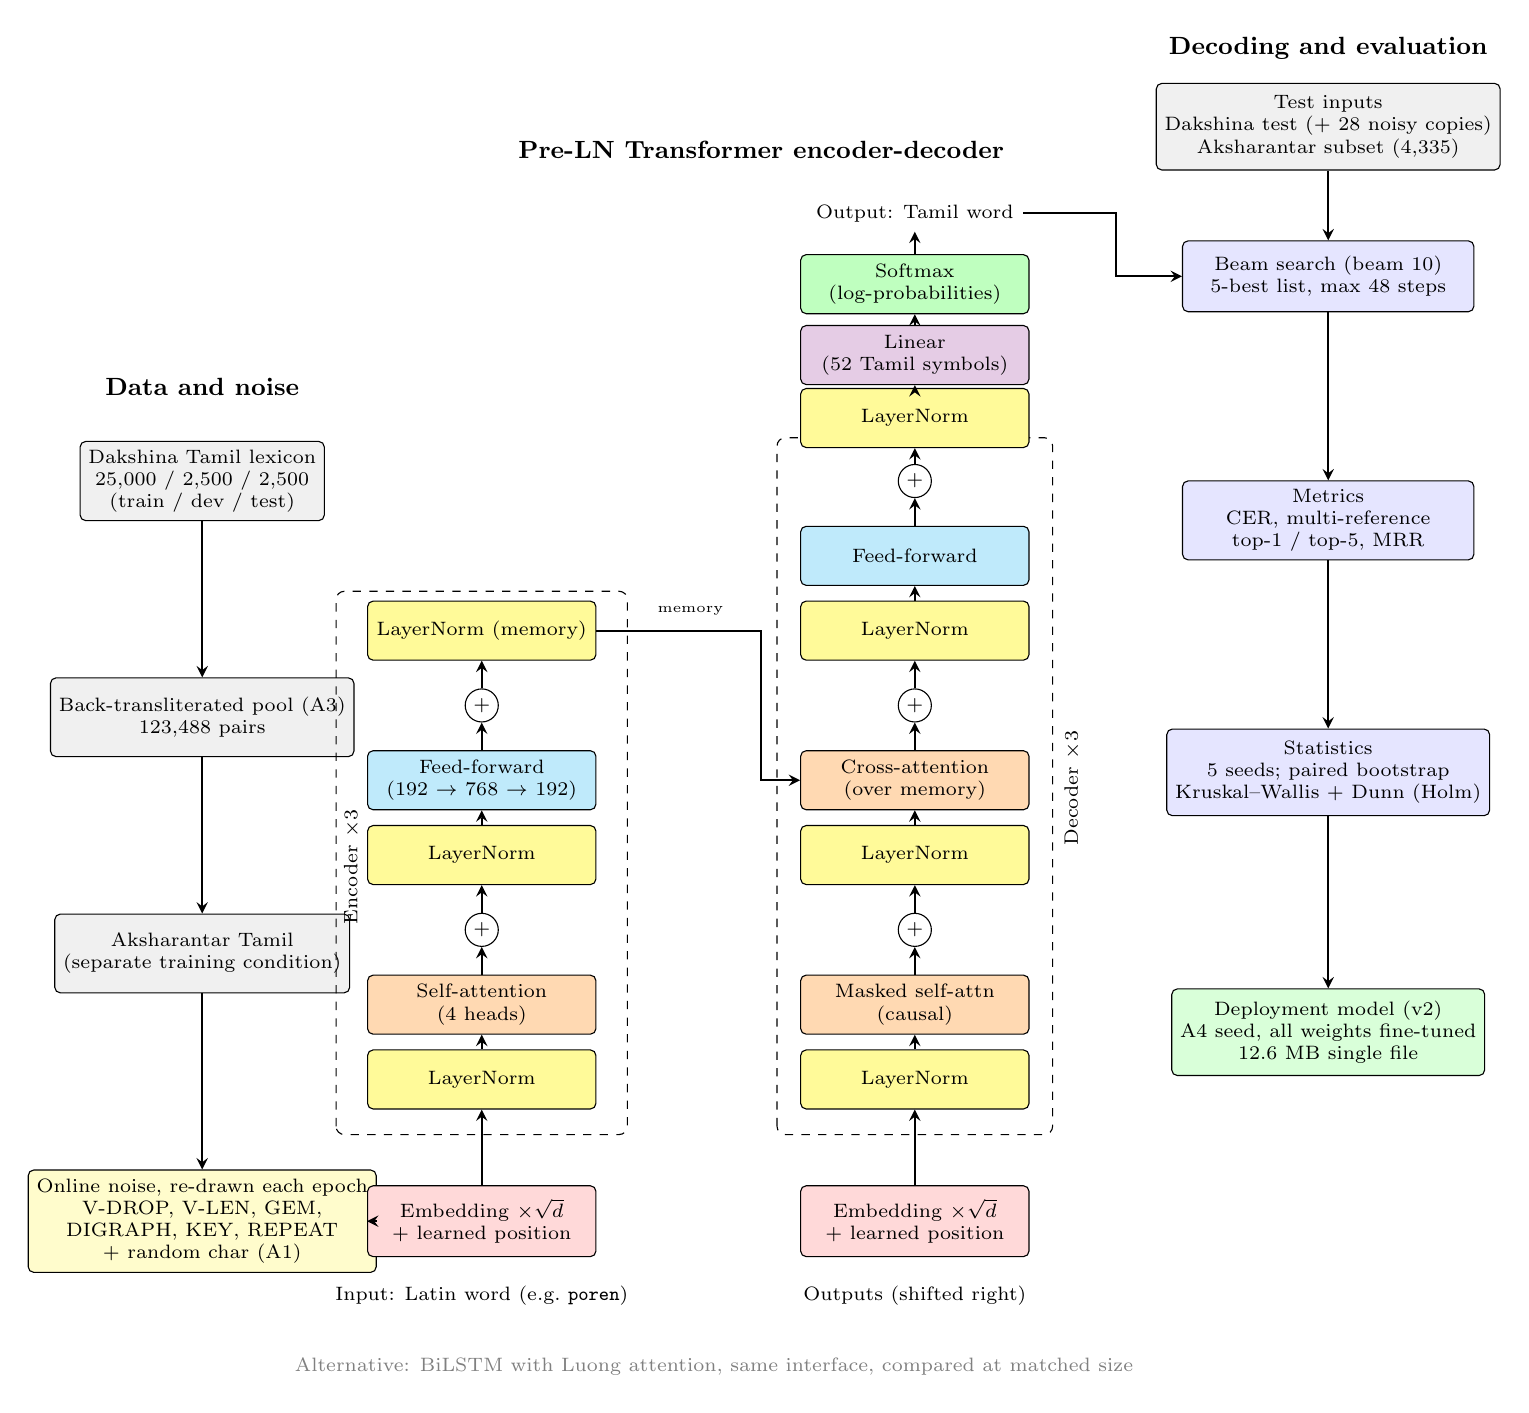
\begin{tikzpicture}[
  blk/.style={draw, rounded corners=2pt, minimum width=2.9cm, minimum height=0.75cm, font=\scriptsize, align=center, inner sep=3pt},
  emb/.style={blk, fill=red!15, minimum height=0.9cm},
  att/.style={blk, fill=orange!30},
  ffn/.style={blk, fill=cyan!25},
  nrm/.style={blk, fill=yellow!40},
  outp/.style={blk, fill=violet!20},
  smx/.style={blk, fill=green!25},
  dat/.style={blk, minimum width=3.0cm, fill=gray!12, minimum height=1.0cm},
  add/.style={circle, draw, inner sep=0pt, minimum size=0.42cm, font=\scriptsize},
  grp/.style={draw, dashed, rounded corners=3pt},
  arr/.style={->, >=stealth, thick},
]

% ---------- Column A: data and noise ----------
\node[font=\small\bfseries] at (1.5,11.6) {Data and noise};
\node[dat] (a1) at (1.5,10.4) {Dakshina Tamil lexicon\\25{,}000 / 2{,}500 / 2{,}500\\(train / dev / test)};
\node[dat] (a2) at (1.5,7.4) {Back-transliterated pool (A3)\\123{,}488 pairs};
\node[dat] (a3) at (1.5,4.4) {Aksharantar Tamil\\(separate training condition)};
\node[dat, minimum height=1.3cm, fill=yellow!20] (a4) at (1.5,1.0) {Online noise, re-drawn each epoch\\V-DROP, V-LEN, GEM,\\DIGRAPH, KEY, REPEAT\\+ random char (A1)};
\draw[arr] (a1) -- (a2);
\draw[arr] (a2) -- (a3);
\draw[arr] (a3) -- (a4);

% ---------- Column B: Transformer encoder-decoder ----------
\node[font=\small\bfseries] at (8.6,14.6) {Pre-LN Transformer encoder-decoder};

% Encoder (source = romanized word)
\node[emb] (e1) at (5.05,1.0) {Embedding $\times\sqrt{d}$\\+ learned position};
\node[nrm] (e2) at (5.05,2.8) {LayerNorm};
\node[att] (e3) at (5.05,3.75) {Self-attention\\(4 heads)};
\node[add] (e4) at (5.05,4.7) {$+$};
\node[nrm] (e5) at (5.05,5.65) {LayerNorm};
\node[ffn] (e6) at (5.05,6.6) {Feed-forward\\(192 $\rightarrow$ 768 $\rightarrow$ 192)};
\node[add] (e7) at (5.05,7.55) {$+$};
\node[nrm] (en) at (5.05,8.5) {LayerNorm (memory)};
\draw[grp] (3.2,2.1) rectangle (6.9,9.0);
\node[rotate=90, font=\scriptsize] at (3.4,5.5) {Encoder $\times 3$};
\draw[arr] (e1) -- (e2);
\draw[arr] (e2) -- (e3);
\draw[arr] (e3) -- (e4);
\draw[arr] (e4) -- (e5);
\draw[arr] (e5) -- (e6);
\draw[arr] (e6) -- (e7);
\draw[arr] (e7) -- (en);

% Decoder (target shifted right, causal)
\node[emb] (d1) at (10.55,1.0) {Embedding $\times\sqrt{d}$\\+ learned position};
\node[nrm] (d2) at (10.55,2.8) {LayerNorm};
\node[att] (d3) at (10.55,3.75) {Masked self-attn\\(causal)};
\node[add] (d4) at (10.55,4.7) {$+$};
\node[nrm] (d4n) at (10.55,5.65) {LayerNorm};
\node[att] (d5) at (10.55,6.6) {Cross-attention\\(over memory)};
\node[add] (d6) at (10.55,7.55) {$+$};
\node[nrm] (d7) at (10.55,8.5) {LayerNorm};
\node[ffn] (d8) at (10.55,9.45) {Feed-forward};
\node[add] (d9) at (10.55,10.4) {$+$};
\draw[grp] (8.8,2.1) rectangle (12.3,10.95);
\node[rotate=90, font=\scriptsize] at (12.55,6.5) {Decoder $\times 3$};
\draw[arr] (d1) -- (d2);
\draw[arr] (d2) -- (d3);
\draw[arr] (d3) -- (d4);
\draw[arr] (d4) -- (d4n);
\draw[arr] (d4n) -- (d5);
\draw[arr] (d5) -- (d6);
\draw[arr] (d6) -- (d7);
\draw[arr] (d7) -- (d8);
\draw[arr] (d8) -- (d9);

% Memory from encoder into decoder cross-attention
\draw[arr] (en.east) -- (8.6,8.5) |- (d5.west);
\node[font=\tiny] at (7.7,8.75) {memory};

% Output head
\node[nrm] (of) at (10.55,11.2) {LayerNorm};
\node[outp] (o1) at (10.55,12.0) {Linear\\(52 Tamil symbols)};
\node[smx] (o2) at (10.55,12.9) {Softmax\\(log-probabilities)};
\node[font=\scriptsize] (o3) at (10.55,13.8) {Output: Tamil word};
\draw[arr] (d9) -- (of);
\draw[arr] (of) -- (o1);
\draw[arr] (o1) -- (o2);
\draw[arr] (o2) -- (o3);

% Inputs
\node[font=\scriptsize] at (5.05,0.05) {Input: Latin word (e.g.\ \texttt{poren})};
\node[font=\scriptsize] at (10.55,0.05) {Outputs (shifted right)};
\draw[arr] (a4.east) -- (e1.west);
\node[font=\scriptsize, text=gray] at (8.0,-0.85) {Alternative: BiLSTM with Luong attention, same interface, compared at matched size};

% ---------- Column C: decoding and evaluation ----------
\node[font=\small\bfseries] at (15.8,15.9) {Decoding and evaluation};
\node[dat, minimum height=1.1cm] (t0) at (15.8,14.9) {Test inputs\\Dakshina test (+ 28 noisy copies)\\Aksharantar subset (4{,}335)};
\node[blk, fill=blue!10, minimum width=3.7cm, minimum height=0.9cm] (c1) at (15.8,13.0) {Beam search (beam 10)\\5-best list, max 48 steps};
\node[blk, fill=blue!10, minimum width=3.7cm, minimum height=1.0cm] (c2) at (15.8,9.9) {Metrics\\CER, multi-reference\\top-1 / top-5, MRR};
\node[blk, fill=blue!10, minimum width=3.7cm, minimum height=1.1cm] (c3) at (15.8,6.7) {Statistics\\5 seeds; paired bootstrap\\Kruskal--Wallis + Dunn (Holm)};
\node[blk, fill=green!15, minimum width=3.7cm, minimum height=1.1cm] (c4) at (15.8,3.4) {Deployment model (v2)\\A4 seed, all weights fine-tuned\\12.6 MB single file};
\draw[arr] (t0) -- (c1);
\draw[arr] (c1) -- (c2);
\draw[arr] (c2) -- (c3);
\draw[arr] (c3) -- (c4);
\draw[arr] (o3.east) -- (13.1,13.8) |- (c1.west);

\end{tikzpicture}%
}
\caption{Architecture of the system. Left: the data sources, and the noise that is re-drawn online each epoch (six Tamil-specific operators, plus random character noise for A1). Centre: the pre-LN Transformer encoder-decoder used in the main comparison (three layers per side, four heads, $d{=}192$, feed-forward width 768, learned positions; 3.15M parameters at the deployment size). Each sublayer is LayerNorm, then the sublayer, then the residual addition ($+$); the encoder output passes through a final LayerNorm to the decoder's cross-attention. Right: test inputs are decoded with beam search (beam 10) and scored; statistics use five seeds and paired bootstrap; the best A4 seed is fine-tuned into the deployment model.}
\label{fig:architecture}
\end{figure*}
